% Options for packages loaded elsewhere
\PassOptionsToPackage{unicode}{hyperref}
\PassOptionsToPackage{hyphens}{url}
%
\documentclass[
]{article}
\usepackage{amsmath,amssymb}
\usepackage{iftex}
\ifPDFTeX
  \usepackage[T1]{fontenc}
  \usepackage[utf8]{inputenc}
  \usepackage{textcomp} % provide euro and other symbols
\else % if luatex or xetex
  \usepackage{unicode-math} % this also loads fontspec
  \defaultfontfeatures{Scale=MatchLowercase}
  \defaultfontfeatures[\rmfamily]{Ligatures=TeX,Scale=1}
\fi
\usepackage{lmodern}
\ifPDFTeX\else
  % xetex/luatex font selection
    \setmainfont[]{NanumGothic}
    \setmonofont[]{UnShinmun}
\fi
% Use upquote if available, for straight quotes in verbatim environments
\IfFileExists{upquote.sty}{\usepackage{upquote}}{}
\IfFileExists{microtype.sty}{% use microtype if available
  \usepackage[]{microtype}
  \UseMicrotypeSet[protrusion]{basicmath} % disable protrusion for tt fonts
}{}
\makeatletter
\@ifundefined{KOMAClassName}{% if non-KOMA class
  \IfFileExists{parskip.sty}{%
    \usepackage{parskip}
  }{% else
    \setlength{\parindent}{0pt}
    \setlength{\parskip}{6pt plus 2pt minus 1pt}}
}{% if KOMA class
  \KOMAoptions{parskip=half}}
\makeatother
\usepackage{xcolor}
\usepackage[margin=1in]{geometry}
\usepackage{color}
\usepackage{fancyvrb}
\newcommand{\VerbBar}{|}
\newcommand{\VERB}{\Verb[commandchars=\\\{\}]}
\DefineVerbatimEnvironment{Highlighting}{Verbatim}{commandchars=\\\{\}}
% Add ',fontsize=\small' for more characters per line
\usepackage{framed}
\definecolor{shadecolor}{RGB}{248,248,248}
\newenvironment{Shaded}{\begin{snugshade}}{\end{snugshade}}
\newcommand{\AlertTok}[1]{\textcolor[rgb]{0.94,0.16,0.16}{#1}}
\newcommand{\AnnotationTok}[1]{\textcolor[rgb]{0.56,0.35,0.01}{\textbf{\textit{#1}}}}
\newcommand{\AttributeTok}[1]{\textcolor[rgb]{0.13,0.29,0.53}{#1}}
\newcommand{\BaseNTok}[1]{\textcolor[rgb]{0.00,0.00,0.81}{#1}}
\newcommand{\BuiltInTok}[1]{#1}
\newcommand{\CharTok}[1]{\textcolor[rgb]{0.31,0.60,0.02}{#1}}
\newcommand{\CommentTok}[1]{\textcolor[rgb]{0.56,0.35,0.01}{\textit{#1}}}
\newcommand{\CommentVarTok}[1]{\textcolor[rgb]{0.56,0.35,0.01}{\textbf{\textit{#1}}}}
\newcommand{\ConstantTok}[1]{\textcolor[rgb]{0.56,0.35,0.01}{#1}}
\newcommand{\ControlFlowTok}[1]{\textcolor[rgb]{0.13,0.29,0.53}{\textbf{#1}}}
\newcommand{\DataTypeTok}[1]{\textcolor[rgb]{0.13,0.29,0.53}{#1}}
\newcommand{\DecValTok}[1]{\textcolor[rgb]{0.00,0.00,0.81}{#1}}
\newcommand{\DocumentationTok}[1]{\textcolor[rgb]{0.56,0.35,0.01}{\textbf{\textit{#1}}}}
\newcommand{\ErrorTok}[1]{\textcolor[rgb]{0.64,0.00,0.00}{\textbf{#1}}}
\newcommand{\ExtensionTok}[1]{#1}
\newcommand{\FloatTok}[1]{\textcolor[rgb]{0.00,0.00,0.81}{#1}}
\newcommand{\FunctionTok}[1]{\textcolor[rgb]{0.13,0.29,0.53}{\textbf{#1}}}
\newcommand{\ImportTok}[1]{#1}
\newcommand{\InformationTok}[1]{\textcolor[rgb]{0.56,0.35,0.01}{\textbf{\textit{#1}}}}
\newcommand{\KeywordTok}[1]{\textcolor[rgb]{0.13,0.29,0.53}{\textbf{#1}}}
\newcommand{\NormalTok}[1]{#1}
\newcommand{\OperatorTok}[1]{\textcolor[rgb]{0.81,0.36,0.00}{\textbf{#1}}}
\newcommand{\OtherTok}[1]{\textcolor[rgb]{0.56,0.35,0.01}{#1}}
\newcommand{\PreprocessorTok}[1]{\textcolor[rgb]{0.56,0.35,0.01}{\textit{#1}}}
\newcommand{\RegionMarkerTok}[1]{#1}
\newcommand{\SpecialCharTok}[1]{\textcolor[rgb]{0.81,0.36,0.00}{\textbf{#1}}}
\newcommand{\SpecialStringTok}[1]{\textcolor[rgb]{0.31,0.60,0.02}{#1}}
\newcommand{\StringTok}[1]{\textcolor[rgb]{0.31,0.60,0.02}{#1}}
\newcommand{\VariableTok}[1]{\textcolor[rgb]{0.00,0.00,0.00}{#1}}
\newcommand{\VerbatimStringTok}[1]{\textcolor[rgb]{0.31,0.60,0.02}{#1}}
\newcommand{\WarningTok}[1]{\textcolor[rgb]{0.56,0.35,0.01}{\textbf{\textit{#1}}}}
\usepackage{graphicx}
\makeatletter
\def\maxwidth{\ifdim\Gin@nat@width>\linewidth\linewidth\else\Gin@nat@width\fi}
\def\maxheight{\ifdim\Gin@nat@height>\textheight\textheight\else\Gin@nat@height\fi}
\makeatother
% Scale images if necessary, so that they will not overflow the page
% margins by default, and it is still possible to overwrite the defaults
% using explicit options in \includegraphics[width, height, ...]{}
\setkeys{Gin}{width=\maxwidth,height=\maxheight,keepaspectratio}
% Set default figure placement to htbp
\makeatletter
\def\fps@figure{htbp}
\makeatother
\setlength{\emergencystretch}{3em} % prevent overfull lines
\providecommand{\tightlist}{%
  \setlength{\itemsep}{0pt}\setlength{\parskip}{0pt}}
\setcounter{secnumdepth}{-\maxdimen} % remove section numbering
\usepackage{fvextra}
\fvset{breaklines}
\ifLuaTeX
  \usepackage{selnolig}  % disable illegal ligatures
\fi
\usepackage{bookmark}
\IfFileExists{xurl.sty}{\usepackage{xurl}}{} % add URL line breaks if available
\urlstyle{same}
\hypersetup{
  pdftitle={Timeseries\_Analysis\_HW1},
  pdfauthor={Na SeungChan},
  hidelinks,
  pdfcreator={LaTeX via pandoc}}

\title{Timeseries\_Analysis\_HW1}
\author{Na SeungChan}
\date{2025-03-28}

\begin{document}
\maketitle

\begin{center}\rule{0.5\linewidth}{0.5pt}\end{center}

\section{10}\label{section}

\begin{Shaded}
\begin{Highlighting}[]
\FunctionTok{set.seed}\NormalTok{(}\DecValTok{42}\NormalTok{)}
\NormalTok{dataX }\OtherTok{\textless{}{-}} \FunctionTok{c}\NormalTok{(}\DecValTok{0}\NormalTok{)}
\NormalTok{dataY }\OtherTok{\textless{}{-}} \FunctionTok{c}\NormalTok{(}\DecValTok{0}\NormalTok{)}
\NormalTok{dataZ }\OtherTok{\textless{}{-}} \FunctionTok{c}\NormalTok{(}\DecValTok{0}\NormalTok{)}
\NormalTok{T }\OtherTok{\textless{}{-}} \DecValTok{10000}
\NormalTok{errors }\OtherTok{\textless{}{-}} \FunctionTok{rnorm}\NormalTok{(T, }\DecValTok{0}\NormalTok{, }\DecValTok{1}\NormalTok{)}

\ControlFlowTok{for}\NormalTok{ (t }\ControlFlowTok{in} \DecValTok{1}\SpecialCharTok{:}\NormalTok{T) \{}
\NormalTok{  dataX }\OtherTok{\textless{}{-}} \FunctionTok{append}\NormalTok{(dataX, dataX[t]}\SpecialCharTok{*}\FloatTok{0.3} \SpecialCharTok{+}\NormalTok{ errors[t])}
\NormalTok{  dataY }\OtherTok{\textless{}{-}} \FunctionTok{append}\NormalTok{(dataY, dataX[t] }\SpecialCharTok{+}\NormalTok{ t)}
\NormalTok{  dataZ }\OtherTok{\textless{}{-}} \FunctionTok{append}\NormalTok{(dataZ, dataX[t] }\SpecialCharTok{+} \FunctionTok{sin}\NormalTok{(t))}
\NormalTok{\}}
\FunctionTok{plot}\NormalTok{(dataX, }\AttributeTok{main =} \StringTok{\textquotesingle{}\{X\_t\}\textquotesingle{}}\NormalTok{, }\AttributeTok{sub =} \StringTok{\textquotesingle{}n=10000\textquotesingle{}}\NormalTok{)}
\end{Highlighting}
\end{Shaded}

\begin{center}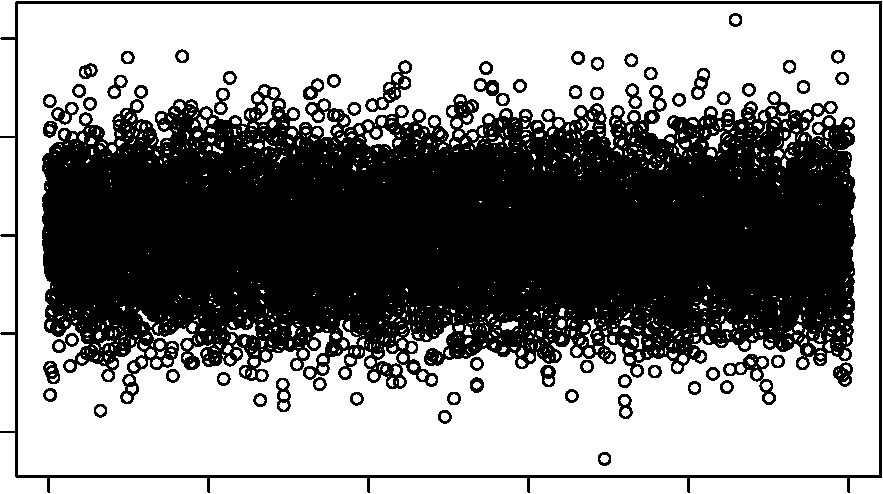
\includegraphics[width=0.8\linewidth]{R_timeseries_HW1_files/figure-latex/unnamed-chunk-1-1} \end{center}

\begin{Shaded}
\begin{Highlighting}[]
\FunctionTok{plot}\NormalTok{(dataY, }\AttributeTok{main =} \StringTok{\textquotesingle{}\{Y\_t\}\textquotesingle{}}\NormalTok{, }\AttributeTok{sub =} \StringTok{\textquotesingle{}n=10000\textquotesingle{}}\NormalTok{)}
\end{Highlighting}
\end{Shaded}

\begin{center}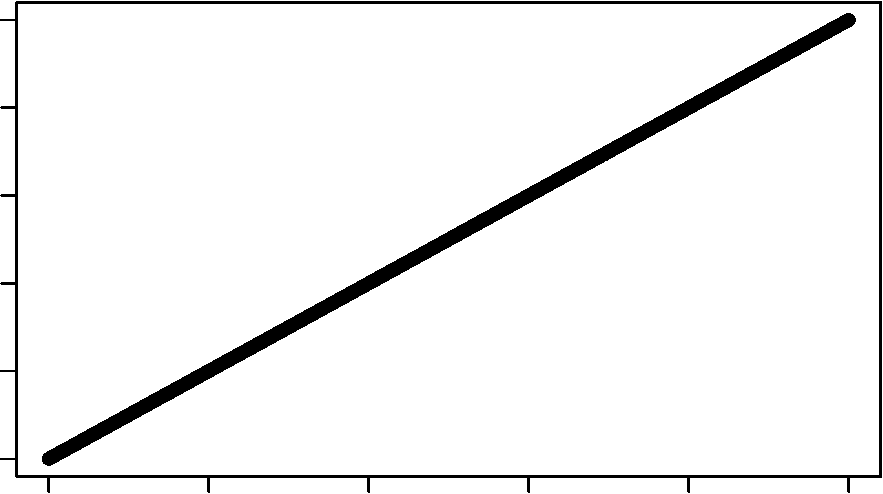
\includegraphics[width=0.8\linewidth]{R_timeseries_HW1_files/figure-latex/unnamed-chunk-1-2} \end{center}

\begin{Shaded}
\begin{Highlighting}[]
\FunctionTok{plot}\NormalTok{(dataZ, }\AttributeTok{main =} \StringTok{\textquotesingle{}\{Z\_t\}\textquotesingle{}}\NormalTok{, }\AttributeTok{sub =} \StringTok{\textquotesingle{}n=10000\textquotesingle{}}\NormalTok{)}
\end{Highlighting}
\end{Shaded}

\begin{center}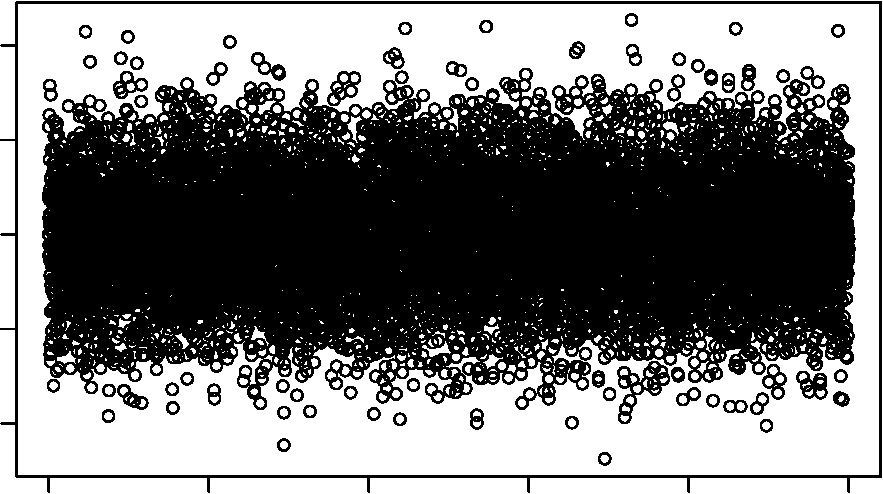
\includegraphics[width=0.8\linewidth]{R_timeseries_HW1_files/figure-latex/unnamed-chunk-1-3} \end{center}

\{X\_t\}는 플롯에 의하면 정상시계열이다. AR(1) 모델이고 그 계수의
절댓값이 1보다 작으므로 정상시계열이 실제 되는 것도 명백하다.

\{Y\_t\}는 시간축 t에 의해 그 값이 좌우되므로 정상시계열이 아니다.

\{Z\_t\}는 정상시계열이 아니지만, sint에 의해 그 변화가 주기적으로
일어나므로 플롯상 정상시계열로 보인다.

\section{11}\label{section-1}

\subsection{(1)}\label{section-2}

\begin{Shaded}
\begin{Highlighting}[]
\NormalTok{name }\OtherTok{\textless{}{-}} \FunctionTok{c}\NormalTok{(}\StringTok{\textquotesingle{}나연\textquotesingle{}}\NormalTok{, }\StringTok{\textquotesingle{}민재\textquotesingle{}}\NormalTok{, }\StringTok{\textquotesingle{}서준\textquotesingle{}}\NormalTok{, }\StringTok{\textquotesingle{}소연\textquotesingle{}}\NormalTok{, }\StringTok{\textquotesingle{}수민\textquotesingle{}}\NormalTok{, }\StringTok{\textquotesingle{}예린\textquotesingle{}}\NormalTok{, }\StringTok{\textquotesingle{}지은\textquotesingle{}}\NormalTok{, }\StringTok{\textquotesingle{}지훈\textquotesingle{}}\NormalTok{, }\StringTok{\textquotesingle{}준호\textquotesingle{}}\NormalTok{, }\StringTok{\textquotesingle{}현우\textquotesingle{}}\NormalTok{)}
\NormalTok{gender }\OtherTok{\textless{}{-}} \FunctionTok{c}\NormalTok{(}\StringTok{\textquotesingle{}여\textquotesingle{}}\NormalTok{, }\StringTok{\textquotesingle{}남\textquotesingle{}}\NormalTok{, }\StringTok{\textquotesingle{}남\textquotesingle{}}\NormalTok{, }\StringTok{\textquotesingle{}여\textquotesingle{}}\NormalTok{, }\StringTok{\textquotesingle{}여\textquotesingle{}}\NormalTok{, }\StringTok{\textquotesingle{}여\textquotesingle{}}\NormalTok{, }\StringTok{\textquotesingle{}여\textquotesingle{}}\NormalTok{, }\StringTok{\textquotesingle{}남\textquotesingle{}}\NormalTok{, }\StringTok{\textquotesingle{}남\textquotesingle{}}\NormalTok{, }\StringTok{\textquotesingle{}남\textquotesingle{}}\NormalTok{)}
\NormalTok{running }\OtherTok{\textless{}{-}} \FunctionTok{c}\NormalTok{(}\FloatTok{14.2}\NormalTok{, }\FloatTok{11.7}\NormalTok{, }\FloatTok{13.8}\NormalTok{, }\FloatTok{15.0}\NormalTok{, }\FloatTok{17.1}\NormalTok{, }\FloatTok{19.5}\NormalTok{, }\FloatTok{13.7}\NormalTok{, }\FloatTok{15.5}\NormalTok{, }\FloatTok{16.3}\NormalTok{, }\FloatTok{12.3}\NormalTok{)}
\NormalTok{palgup }\OtherTok{\textless{}{-}} \FunctionTok{c}\NormalTok{(}\DecValTok{38}\NormalTok{, }\DecValTok{51}\NormalTok{, }\DecValTok{48}\NormalTok{, }\DecValTok{27}\NormalTok{, }\DecValTok{9}\NormalTok{, }\DecValTok{13}\NormalTok{, }\DecValTok{37}\NormalTok{, }\DecValTok{55}\NormalTok{, }\DecValTok{45}\NormalTok{, }\DecValTok{19}\NormalTok{)}

\NormalTok{physical\_test }\OtherTok{\textless{}{-}} \FunctionTok{data.frame}\NormalTok{(name, gender, running, palgup)}
\end{Highlighting}
\end{Shaded}

\subsection{(2)}\label{section-3}

\begin{Shaded}
\begin{Highlighting}[]
\NormalTok{solo\_rating }\OtherTok{\textless{}{-}} \ControlFlowTok{function}\NormalTok{(gndr, run, pal)\{}
  \ControlFlowTok{if}\NormalTok{ (gndr }\SpecialCharTok{==} \StringTok{\textquotesingle{}여\textquotesingle{}}\NormalTok{) \{}
\NormalTok{    run\_score }\OtherTok{\textless{}{-}} \FunctionTok{case\_when}\NormalTok{(}
\NormalTok{    run }\SpecialCharTok{\textgreater{}=} \FloatTok{18.0} \SpecialCharTok{\textasciitilde{}} \DecValTok{0}\NormalTok{,}
\NormalTok{    run }\SpecialCharTok{\textgreater{}=} \FloatTok{16.0} \SpecialCharTok{\textasciitilde{}} \DecValTok{1}\NormalTok{,}
\NormalTok{    run }\SpecialCharTok{\textgreater{}} \FloatTok{14.0} \SpecialCharTok{\textasciitilde{}} \DecValTok{2}\NormalTok{,}
    \ConstantTok{TRUE} \SpecialCharTok{\textasciitilde{}} \DecValTok{3}
\NormalTok{    )}
\NormalTok{    pal\_score }\OtherTok{\textless{}{-}} \FunctionTok{case\_when}\NormalTok{(}
\NormalTok{    pal }\SpecialCharTok{\textless{}=} \DecValTok{9} \SpecialCharTok{\textasciitilde{}} \DecValTok{0}\NormalTok{,}
\NormalTok{    pal }\SpecialCharTok{\textless{}=} \DecValTok{19} \SpecialCharTok{\textasciitilde{}} \DecValTok{1}\NormalTok{,}
\NormalTok{    pal }\SpecialCharTok{\textless{}=} \DecValTok{34} \SpecialCharTok{\textasciitilde{}} \DecValTok{2}\NormalTok{,}
    \ConstantTok{TRUE} \SpecialCharTok{\textasciitilde{}} \DecValTok{3}
\NormalTok{    )\} }
    \ControlFlowTok{else} \ControlFlowTok{if}\NormalTok{ (gndr }\SpecialCharTok{==} \StringTok{\textquotesingle{}남\textquotesingle{}}\NormalTok{) \{}
\NormalTok{    run\_score }\OtherTok{\textless{}{-}} \FunctionTok{case\_when}\NormalTok{(}
\NormalTok{    run }\SpecialCharTok{\textgreater{}=} \FloatTok{16.1} \SpecialCharTok{\textasciitilde{}} \DecValTok{0}\NormalTok{,}
\NormalTok{    run }\SpecialCharTok{\textgreater{}=} \FloatTok{14.1} \SpecialCharTok{\textasciitilde{}} \DecValTok{1}\NormalTok{,}
\NormalTok{    run }\SpecialCharTok{\textgreater{}} \FloatTok{12.1} \SpecialCharTok{\textasciitilde{}} \DecValTok{2}\NormalTok{,}
    \ConstantTok{TRUE} \SpecialCharTok{\textasciitilde{}} \DecValTok{3}
\NormalTok{    )}
\NormalTok{    pal\_score }\OtherTok{\textless{}{-}} \FunctionTok{case\_when}\NormalTok{(}
\NormalTok{    pal }\SpecialCharTok{\textless{}=} \DecValTok{19} \SpecialCharTok{\textasciitilde{}} \DecValTok{0}\NormalTok{,}
\NormalTok{    pal }\SpecialCharTok{\textless{}=} \DecValTok{34} \SpecialCharTok{\textasciitilde{}} \DecValTok{1}\NormalTok{,}
\NormalTok{    pal }\SpecialCharTok{\textless{}=} \DecValTok{49} \SpecialCharTok{\textasciitilde{}} \DecValTok{2}\NormalTok{,}
    \ConstantTok{TRUE} \SpecialCharTok{\textasciitilde{}} \DecValTok{3}
\NormalTok{    )\}}
  \FunctionTok{return}\NormalTok{(run\_score }\SpecialCharTok{+}\NormalTok{ pal\_score)}
\NormalTok{\}}

\NormalTok{ratings }\OtherTok{\textless{}{-}} \ControlFlowTok{function}\NormalTok{(df)\{}
\NormalTok{  rtlst }\OtherTok{\textless{}{-}} \FunctionTok{c}\NormalTok{()}
  \ControlFlowTok{for}\NormalTok{ (i }\ControlFlowTok{in} \DecValTok{1}\SpecialCharTok{:}\FunctionTok{nrow}\NormalTok{(df)) \{}
\NormalTok{    rtlst }\OtherTok{\textless{}{-}} \FunctionTok{append}\NormalTok{(rtlst, }\FunctionTok{solo\_rating}\NormalTok{(df[i, }\DecValTok{2}\NormalTok{], df[i, }\DecValTok{3}\NormalTok{], df[i, }\DecValTok{4}\NormalTok{]))}
\NormalTok{  \}}
  \FunctionTok{return}\NormalTok{(rtlst)}
\NormalTok{\}}
\end{Highlighting}
\end{Shaded}

\subsection{(3)}\label{section-4}

\begin{Shaded}
\begin{Highlighting}[]
\NormalTok{final\_column }\OtherTok{\textless{}{-}} \FunctionTok{ratings}\NormalTok{(physical\_test)}
\NormalTok{final\_column}
\end{Highlighting}
\end{Shaded}

\begin{verbatim}
##  [1] 5 6 4 4 1 1 6 4 2 2
\end{verbatim}

\begin{Shaded}
\begin{Highlighting}[]
\NormalTok{physical\_test[}\StringTok{\textquotesingle{}스코어\textquotesingle{}}\NormalTok{] }\OtherTok{\textless{}{-}}\NormalTok{ final\_column}
\NormalTok{physical\_test}
\end{Highlighting}
\end{Shaded}

\begin{verbatim}
##    name gender running palgup 스코어
## 1  나연     여    14.2     38      5
## 2  민재     남    11.7     51      6
## 3  서준     남    13.8     48      4
## 4  소연     여    15.0     27      4
## 5  수민     여    17.1      9      1
## 6  예린     여    19.5     13      1
## 7  지은     여    13.7     37      6
## 8  지훈     남    15.5     55      4
## 9  준호     남    16.3     45      2
## 10 현우     남    12.3     19      2
\end{verbatim}

\end{document}
